\begin{figure}[t]
  \centering
  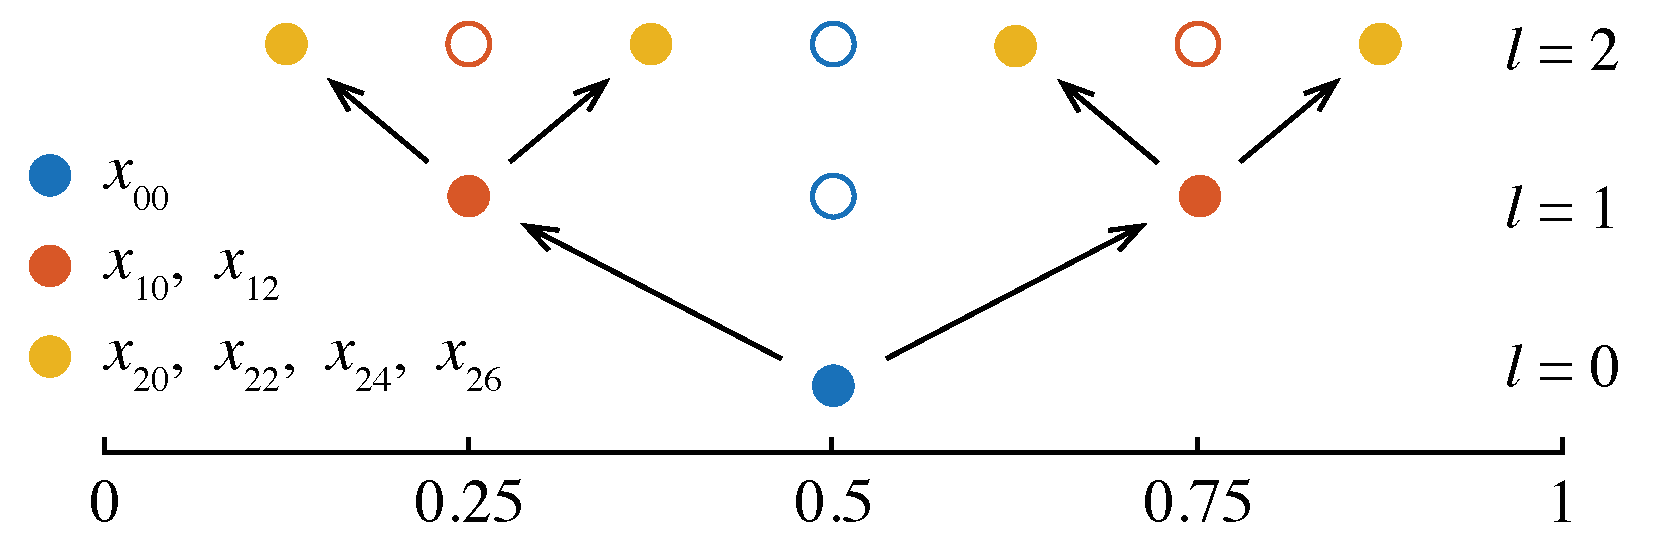
\includegraphics[width=1.0\columnwidth]{include/assets/figures/grid.pdf}
  \vspace{-1em}
  \caption{
    An illustration of the open Newton--Cotes rule. On each level, the dots
    correspond to the nodes introduced by that particular level, and the holes
    correspond to the nodes inherited from the previous levels.
  }
  \flab{grid}
\end{figure}
